\section{Design}

Given the scope of the practical, simplicity was the main goal when designing the RDT protocol. This section will discuss design decisions and rationale behind them. The two attempted extension features, checksums and adaptive re-transmission timeouts,  are also detailed here.

\subsection{Packet Structure}

RDT packets (see Figure~\ref{fig:packet}) are composed of a constant 12 byte header and an optional data segment. The size of the data segment ranges from 0 to 1300 bytes, with 1300 bytes used as the maximum size so as to allow testing with \code{slurpe-3} without issue. Given that the TCP Maximum Segment Size (MSS)~\cite{rfc793} is generally 1500 bytes, this was considered a reasonable choice. Larger packet sizes may also lead to fragmentation at the IP Layer, which was undesirable.

\begin{figure}[h]
\begin{verbatim}
+-+-+-+-+-+-+-+-+-+-+-+-+-+-+-+-+-+-+-+-+-+-+-+-+-+-+-+-+-+-+-+-+
|   Header (12 Bytes)   |         Data (0 - 1300 Bytes)         |
+-+-+-+-+-+-+-+-+-+-+-+-+-+-+-+-+-+-+-+-+-+-+-+-+-+-+-+-+-+-+-+-+
\end{verbatim}
\caption{RDT Packet Structure}\label{fig:packet}
\end{figure}

The RDT header (see Figure~\ref{fig:header}) is comprised of the following fields: a 32-bit \code{sequence} field, used for keeping track of the number of bytes sent by the client; a 16-bit \code{type} field, used to denote the packet function; a 16-bit \code{checksum} field, calculated over the header and data segment to detect bit-errors; a 16-bit \code{size} field denoting the size of the data segment (in bytes); and a 16-bit \code{padding} field to ensure 32-bit word alignment.

Several factors influenced the RDT header design. As file sizes are often calculated as 32-bit integers (such as bythe C library function \code{ftell}), a 32-bit \code{sequence} field was required to support the transmission of large files/amounts of data. For checksums, the given implentation of the IPv4 header checksum used returns a \code{uint16\char`_t} value, thus necessitating a 16-bit field. As a maximum data segment size of 1300 bytes was required, at least 11 bits were required for the \code{size} field, however 16 bits were used for alignment. For the remaining \code{type} and \code{padding} fields, there were no other considerations for field size other than 32-bit alignment. 

\begin{figure}
\begin{center}
\begin{verbatim}
 0                   1                   2                   3  
 0 1 2 3 4 5 6 7 8 9 0 1 2 3 4 5 6 7 8 9 0 1 2 3 4 5 6 7 8 9 0 1
+-+-+-+-+-+-+-+-+-+-+-+-+-+-+-+-+-+-+-+-+-+-+-+-+-+-+-+-+-+-+-+-+
|                            Sequence                           |
+-+-+-+-+-+-+-+-+-+-+-+-+-+-+-+-+-+-+-+-+-+-+-+-+-+-+-+-+-+-+-+-+
|              Type             |            Checksum           |
+-+-+-+-+-+-+-+-+-+-+-+-+-+-+-+-+-+-+-+-+-+-+-+-+-+-+-+-+-+-+-+-+
|              Size             |            Padding            |
+-+-+-+-+-+-+-+-+-+-+-+-+-+-+-+-+-+-+-+-+-+-+-+-+-+-+-+-+-+-+-+-+
\end{verbatim}
\end{center}
\caption{RDT Header}\label{fig:header}
\end{figure}

A single \code{type} field was chosen, rather than a set TCP-style flags, for simplicity. Given the minimal nature of the RDT protocol, it was faster simpler to enumerate all packet types (see below), rather than testing multiple flags.

The type field supports the following types: \code{SYN} (0) and \code{SYN ACK} (1), used for the connection handshake; \code{DATA} (2) and \code{ACK} (3), used for sending and acknowledging data segments; \code{FIN} (4) and \code{FIN ACK} (5), used for graceful connection termination; and \code{RST} (6), used for abrupt connection termination.

\subsection{Connection Management}

The operation of the RDT protocol can be modelled by the FSM in Figure~\ref{fig:fsm}. For connection management, a two-way handshake is used. As RDT only supports uni-directional communication, a two-way handshake (see Figure~\ref{fig:timeline}) is adequate for establishing and terminating connections. Adaptive re-transmission timeouts are used in both the handshakes and transmission of data segments.

During handshakes, timeouts are used, with an initial RTO value of 200ms. This is doubled successively (Section~\ref{sec:RTO}). After 5 timeouts, the client with aborts with an \code{RST} to prevent clients waiting on unavailable hosts or a dropped \code{FIN ACK}.

\subsection{Data Transfer}

RDT uses an Idle-RQ mechanism for sending data segments, and will wait for acknowledgement of each sent segment. If the sender receives an \code{ACK} with a sequence number that is greater than expected or an RTO is triggered, it will retransmit the same packet. If it receives an \code{ACK} with a sequence number lower than expected, it will retransmit from that segment as it assumes a data segment has been dropped or corrupted\dots

For the handshake, a random sequence number is chosen to prevent `old' or `stale' packets from causing errors, and to reduce predictability that could be exploited. The method for generating initial sequence numbers is pseudo-random and not cryptograhically secure. 

\subsection{Adaptive RTO}\label{sec:RTO}
As an extension, adaptive re-transmission timeouts using measured RTT has been implemented. RDT's adaptive RDT is modelled on TCP's Retranmission Timer~\cite{rfc6298}~\endnote{Clock granularity is not considered, however RTO values are calculated in microseconds and the School Lab PCs have a granularity of 1 nanosecond.}, with the same initial RTO of 1s and maximum of 60s.

\begin{figure}[H]
\begin{center}
    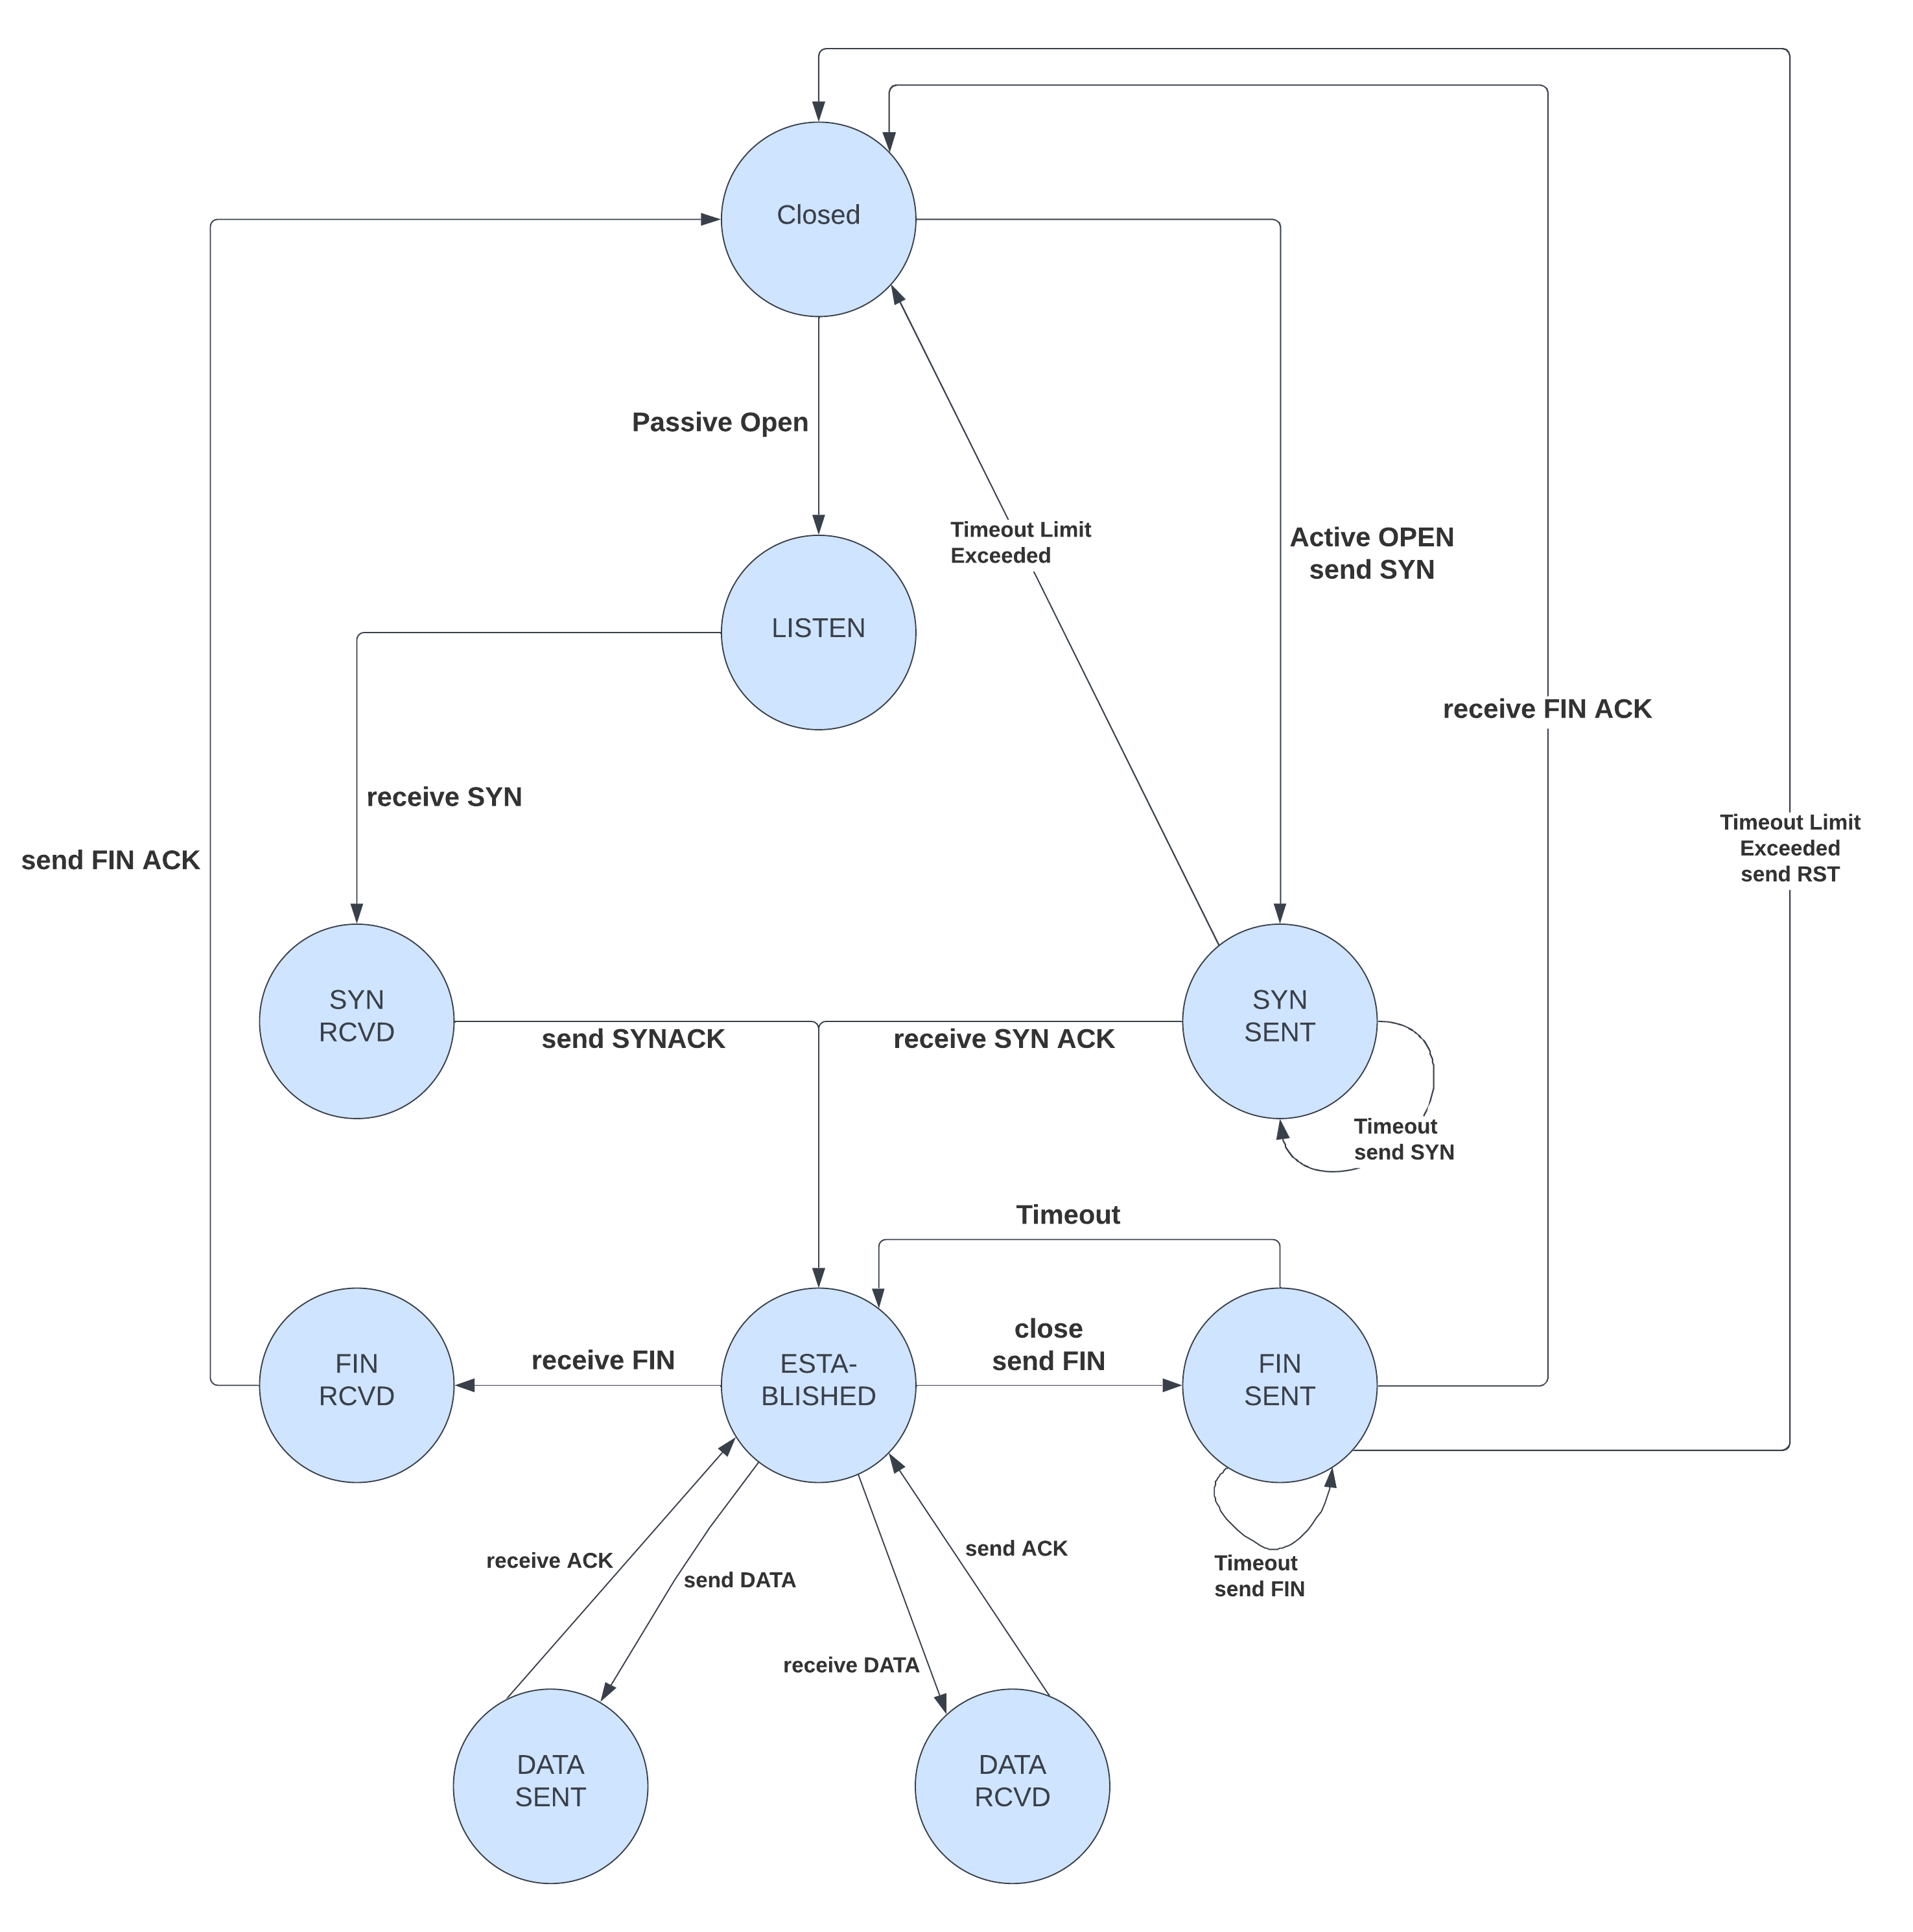
\includegraphics[width=100mm]{images/fsm.png}
\end{center}
\caption{RDT Finite State Machine (see also A.1)}\label{fig:fsm}
\end{figure}

\begin{figure}[h]
\begin{center}
    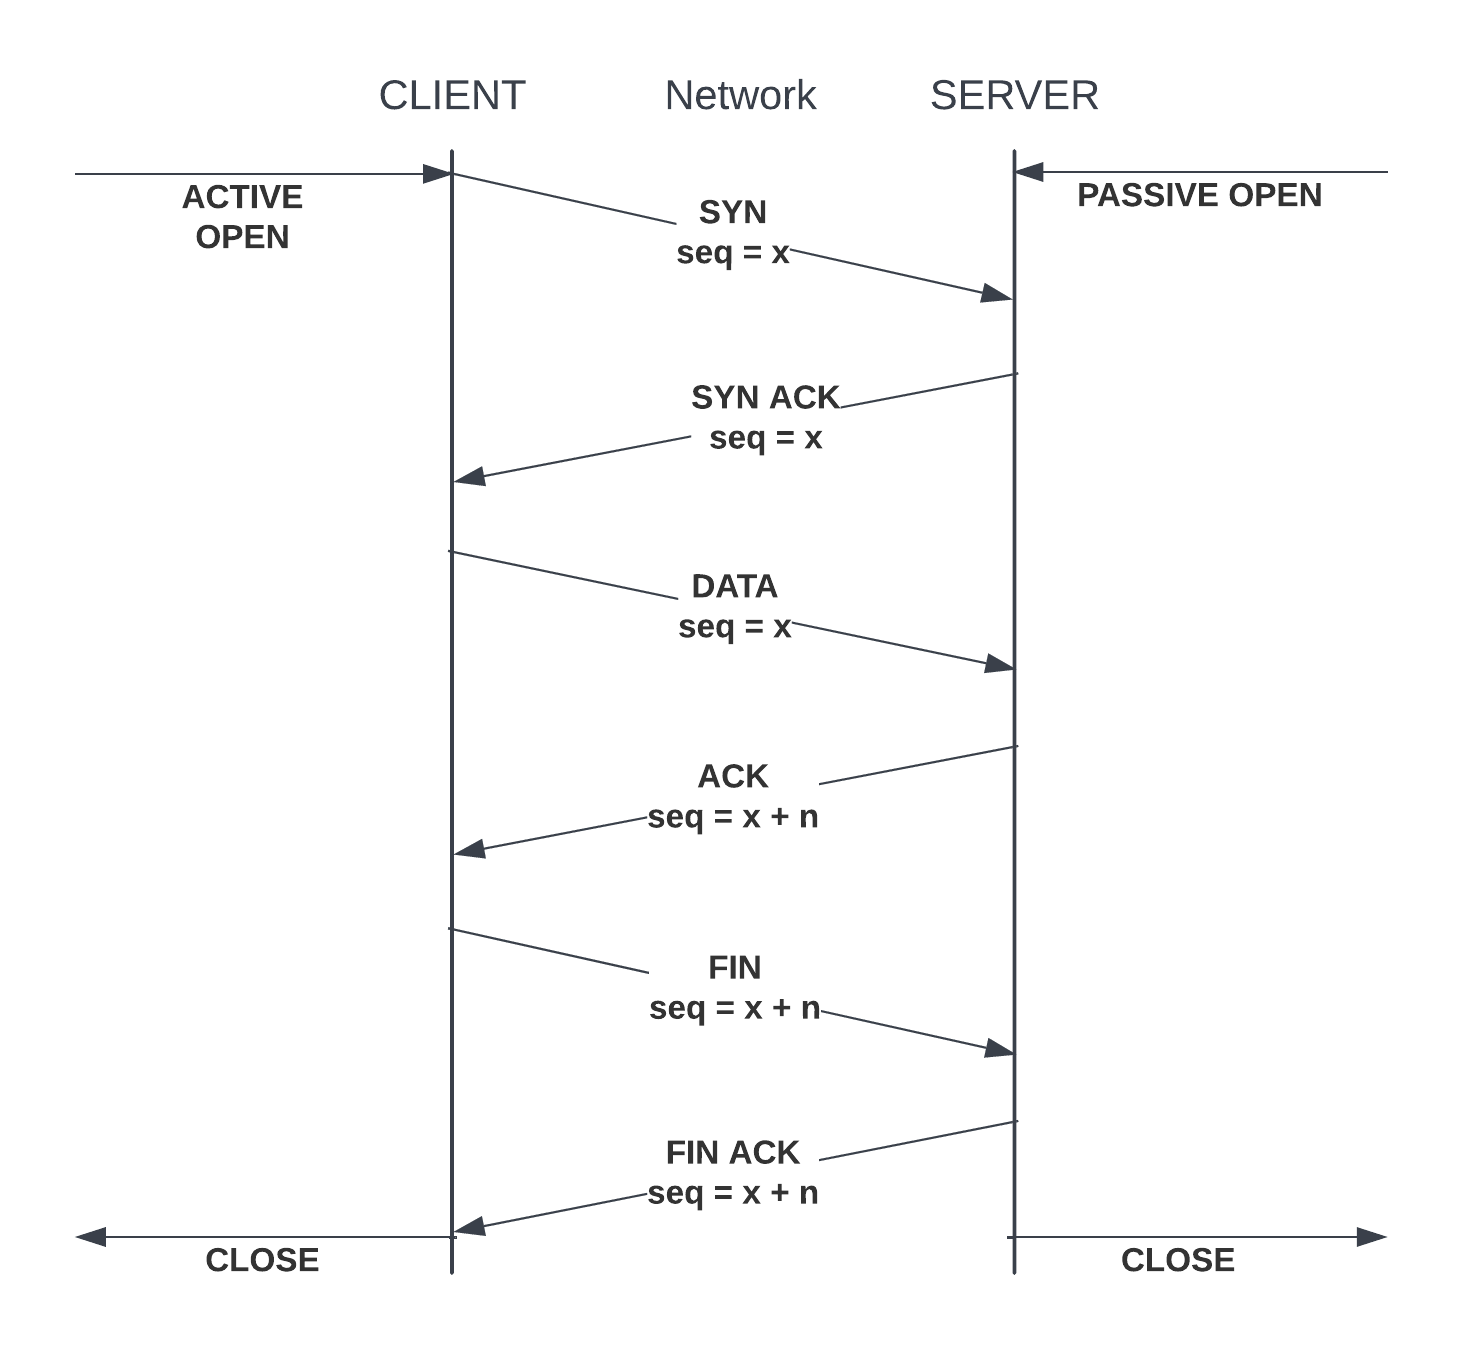
\includegraphics[width=100mm]{images/timeline.png}
\end{center}
\caption{Connection Timeline Diagram (see also A.2)}\label{fig:timeline}
\end{figure} 


\subsection{Checksums}
The RDT \code{checksum} field is calculated over the entire segment/packet (i.e.~header and data) using the IPv4 Header Checksum Algorithm~\cite{rfc791}. The implementation of the original source~\cite{ipv4_checksum} to support the use of 8-bit byte values in the data segment. During checksum calculating, the \code{checksum} field itself is set to 0 for consistency.